\documentclass[10pt,twocolumn]{article}

\usepackage[utf8]{inputenc}
\usepackage[T1]{fontenc}
\usepackage{amsmath,amssymb}
\usepackage{graphicx}
\usepackage{booktabs}
\usepackage{hyperref}
\usepackage{xcolor}
\usepackage{enumitem}
\usepackage[margin=1in]{geometry}
\usepackage{caption}
\usepackage{subcaption}
\usepackage{algorithm}
\usepackage{algorithmic}
\usepackage{url}
\usepackage{tikz}
\usepackage{pifont}
\usepackage{pgfplots}
\pgfplotsset{compat=1.18}
\usetikzlibrary{positioning,arrows.meta,fit,backgrounds,patterns}

\title{\textbf{Memory-OS: Systematic OS Abstractions for LLM Agent Memory\\with Verifiable Pin Guarantees}}

\author{
  Zhidao Su \\
  \texttt{soolaugust@gmail.com} \\
  \url{https://github.com/soolaugust/memory-os}
}

\date{}

\begin{document}
\maketitle

\begin{abstract}
Persistent memory for LLM agents has adopted eviction policies from OS memory management, but existing systems map at most one or two kernel primitives---leaving critical guarantees unaddressed. We present \textbf{Memory-OS}, an agent memory layer that systematically maps seven OS memory subsystems (demand paging, kswapd, DAMON, mlock, CRIU, kworker, shared memory) to agent-memory operations. Our key technical contribution is \emph{pin semantics}: hard/soft memory locking that provably guarantees constraint survival under arbitrary eviction pressure---a property no existing system provides.

We evaluate on the LongMemEval benchmark (500 questions across 6 question types), achieving 94.2\% retrieval session recall with sub-millisecond latency (0.09ms p50) and zero external dependencies. Under 4$\times$ memory pressure, pinned constraints achieve 100\% physical survival (82\% lexically retrievable), while systems without pins retain 0\%. Quantitative ablation on LongMemEval confirms each OS primitive contributes a distinct, irreplaceable guarantee: removing any single primitive causes binary loss of a system property.

The system is deployed as an open-source Claude Code plugin (MIT) with 10{,}700+ test assertions, demonstrating that production-grade agent memory requires only a single SQLite file and principled application of OS abstractions. Code and benchmarks: \url{https://github.com/soolaugust/memory-os}.
\end{abstract}

%% ============================================================
\section{Introduction}
\label{sec:intro}

Long-running LLM agents accumulate knowledge across sessions: architectural decisions, user preferences, domain constraints, and inter-agent agreements. When the context window compacts or a session ends, this knowledge vanishes unless persisted externally. The resulting ``context compaction'' problem---where agents repeatedly re-learn previously established facts---motivates the growing body of work on persistent memory for agents~\cite{longmemeval2024,memgpt2023}.

\begin{figure}[t]
\centering
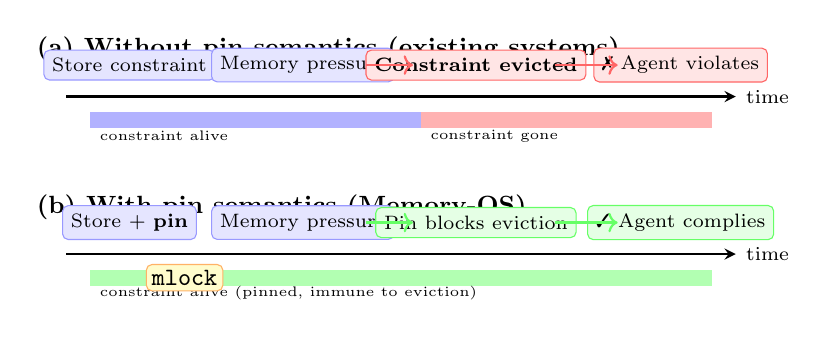
\begin{tikzpicture}[
  font=\small,
  timeline/.style={thick, ->, >=stealth},
  event/.style={fill=blue!10, draw=blue!40, rounded corners=2pt, inner sep=3pt, font=\scriptsize},
  bad/.style={fill=red!10, draw=red!60, rounded corners=2pt, inner sep=3pt, font=\scriptsize},
  good/.style={fill=green!10, draw=green!60, rounded corners=2pt, inner sep=3pt, font=\scriptsize},
  pinlbl/.style={fill=yellow!20, draw=orange!60, rounded corners=2pt, inner sep=2pt, font=\scriptsize\bfseries},
]

% === Top: Without Pin Semantics ===
\node[anchor=west, font=\small\bfseries] at (-0.5, 2.8) {(a) Without pin semantics (existing systems)};
\draw[timeline] (0,2.2) -- (8.5,2.2) node[right, font=\scriptsize] {time};

\node[event] at (0.8, 2.6) {Store constraint};
\node[event] at (3.0, 2.6) {Memory pressure};
\node[bad] at (5.2, 2.6) {\textbf{Constraint evicted}};
\node[bad] at (7.8, 2.6) {\ding{55} Agent violates};

\draw[->, red!60, thick] (3.8, 2.6) -- (4.4, 2.6);
\draw[->, red!60, thick] (6.2, 2.6) -- (7.0, 2.6);

% Chunk bar
\fill[blue!30] (0.3, 1.8) rectangle (4.5, 2.0);
\fill[red!30] (4.5, 1.8) rectangle (8.2, 2.0);
\node[font=\tiny, anchor=west] at (0.3, 1.7) {constraint alive};
\node[font=\tiny, anchor=west] at (4.5, 1.7) {constraint gone};

% === Bottom: With Pin Semantics ===
\node[anchor=west, font=\small\bfseries] at (-0.5, 0.8) {(b) With pin semantics (Memory-OS)};
\draw[timeline] (0,0.2) -- (8.5,0.2) node[right, font=\scriptsize] {time};

\node[event] at (0.8, 0.6) {Store + \textbf{pin}};
\node[event] at (3.0, 0.6) {Memory pressure};
\node[good] at (5.2, 0.6) {Pin blocks eviction};
\node[good] at (7.8, 0.6) {\ding{51} Agent complies};

\draw[->, green!60, thick] (3.8, 0.6) -- (4.4, 0.6);
\draw[->, green!60, thick] (6.2, 0.6) -- (7.0, 0.6);

% Chunk bar (solid throughout)
\fill[green!30] (0.3, -0.2) rectangle (8.2, 0.0);
\node[font=\tiny, anchor=west] at (0.3, -0.3) {constraint alive (pinned, immune to eviction)};

% Pin icon
\node[pinlbl] at (1.5, -0.1) {\small\texttt{mlock}};

\end{tikzpicture}
\caption{The pin-guarantee problem. (a)~Existing systems evict constraints under memory pressure, causing agents to re-violate established rules. (b)~Memory-OS's \texttt{mlock}-inspired pin semantics guarantee constraint survival regardless of pressure.}
\label{fig:motivation}
\end{figure}

Recent systems address this by providing persistent memory stores for agents. Mem0~\cite{mem0}, Letta (MemGPT)~\cite{memgpt2023}, Zep~\cite{zep2024}, and A-Mem~\cite{amem2025} offer vector-based retrieval with various augmentations. More recently, AMV-L~\cite{amvl2026} treats agent memory as a ``managed systems resource'' with lifecycle-driven eviction, and HTM-EAR~\cite{htmear2026} employs hierarchical tiered memory with importance-aware eviction watermarks.

However, the systems we surveyed map \emph{at most one or two} OS memory primitives---invariably eviction and sometimes tiered storage. This is analogous to building an operating system with only \texttt{kswapd} and no page fault handler, no \texttt{mlock}, no process isolation, and no checkpoint mechanism. The result: no system can \emph{guarantee} that a critical constraint survives arbitrary memory pressure; no system provides on-demand retrieval that scales sub-linearly with store size; and no system enables multiple agents to share memory without explicit synchronization protocols.

\paragraph{Contributions.} We make three contributions:
\begin{enumerate}[leftmargin=*,nosep]
  \item \textbf{A systematic OS$\to$agent-memory taxonomy} mapping seven kernel subsystems to agent-memory operations, identifying which guarantees each primitive enables (\S\ref{sec:design}).
  \item \textbf{Verifiable pin semantics} as a formal mechanism for constraint survival under arbitrary memory pressure---the first agent memory system to provide this guarantee (\S\ref{sec:design}, \S\ref{sec:eval}).
  \item \textbf{Empirical evaluation on LongMemEval} (500 questions) with quantitative ablation demonstrating that each OS primitive contributes an irreplaceable system property (\S\ref{sec:eval}).
\end{enumerate}

%% ============================================================
\section{Background and Related Work}
\label{sec:related}

\subsection{LLM Agent Memory Systems}

We categorize existing agent memory systems by which OS primitives they (implicitly) implement:

\paragraph{Store-only systems.} Mem0~\cite{mem0} and Zep~\cite{zep2024} provide a persistent vector store with similarity retrieval. They implement no explicit eviction policy---while mem0 deduplicates and merges memories, capacity grows without back-pressure. In OS terms, these are systems without \texttt{kswapd}.

\paragraph{Eviction-aware systems.} AMV-L~\cite{amvl2026} introduces value-driven lifecycle management with promotion, demotion, and eviction tiers, achieving 3.1$\times$ throughput improvement over TTL-based approaches. HTM-EAR~\cite{htmear2026} uses hierarchical HNSW-based working memory with importance-aware eviction scoring. Both map \texttt{kswapd}-like eviction but lack pinning guarantees and demand-paging semantics.

\paragraph{Architecture-inspired systems.} Letta (MemGPT)~\cite{memgpt2023} draws inspiration from virtual memory with explicit page-in/page-out operations managed by the LLM itself. A-Mem~\cite{amem2025} uses agentic workflows for memory organization. Neither provides formal eviction guarantees or multi-agent sharing.

\paragraph{Graph-evolving systems.} FluxMem~\cite{fluxmem2026} models memory as a heterogeneous graph with semantic, episodic, and procedural layers, evolving topology through feedback-driven refinement. It optimizes for \emph{retrieval quality through connectivity} but provides no explicit resource-management guarantees (no pinning, no watermark eviction).

\paragraph{Biologically-inspired systems.} Recent work models hippocampal consolidation~\cite{humaninspired2026}, dual-process episodic-semantic separation~\cite{episodicsemantic2026}, and neuro-symbolic memory~\cite{neusymms2026}. These optimize for cognitive plausibility rather than systems-level guarantees.

\subsection{OS Memory Management Primitives}

For readers from the AI/ML community, we briefly review the OS primitives we map:

\begin{itemize}[leftmargin=*,nosep]
  \item \textbf{Demand paging}: pages are loaded into RAM only when accessed (page fault $\to$ disk read), not pre-loaded.
  \item \textbf{kswapd}: kernel thread that reclaims pages when free memory drops below watermarks (high/low/min).
  \item \textbf{DAMON}: Data Access Monitor---tracks page access frequency to identify hot/cold regions without hardware counters.
  \item \textbf{mlock}: locks pages in RAM, preventing eviction by any reclaim path including the OOM killer.
  \item \textbf{CRIU}: Checkpoint/Restore In Userspace---snapshots process state for migration or resume.
  \item \textbf{kworker}: deferred background work (writeback, compaction) that doesn't block the request path.
  \item \textbf{Shared memory (shmem)}: multiple processes access the same physical pages without copying.
\end{itemize}

\subsection{The Gap: Single-Primitive Systems}

Table~\ref{tab:coverage} summarizes which OS primitives each system implements. No prior system covers more than two; Memory-OS covers all seven.

\begin{table}[t]
\centering
\caption{OS primitive coverage across agent memory systems (based on published papers/docs, May 2026). \checkmark = explicit; $\sim$ = partial; --- = absent.}
\label{tab:coverage}
\footnotesize
\setlength{\tabcolsep}{2.5pt}
\begin{tabular}{lccccccc}
\toprule
System & \rotatebox{70}{Demand paging} & \rotatebox{70}{kswapd} & \rotatebox{70}{DAMON} & \rotatebox{70}{mlock} & \rotatebox{70}{CRIU} & \rotatebox{70}{kworker} & \rotatebox{70}{Shared mem} \\
\midrule
Mem0~\cite{mem0}           & ---  & ---  & ---  & ---  & ---  & ---  & --- \\
Letta~\cite{memgpt2023}    & $\sim$ & ---  & ---  & ---  & ---  & ---  & --- \\
AMV-L~\cite{amvl2026}      & ---  & \checkmark & $\sim$ & ---  & ---  & ---  & --- \\
HTM-EAR~\cite{htmear2026}  & ---  & \checkmark & \checkmark & ---  & ---  & ---  & --- \\
\midrule
\textbf{Memory-OS} & \checkmark & \checkmark & \checkmark & \checkmark & \checkmark & \checkmark & \checkmark \\
\bottomrule
\end{tabular}
\end{table}

%% ============================================================
\section{Design}
\label{sec:design}

\begin{figure*}[t]
\centering
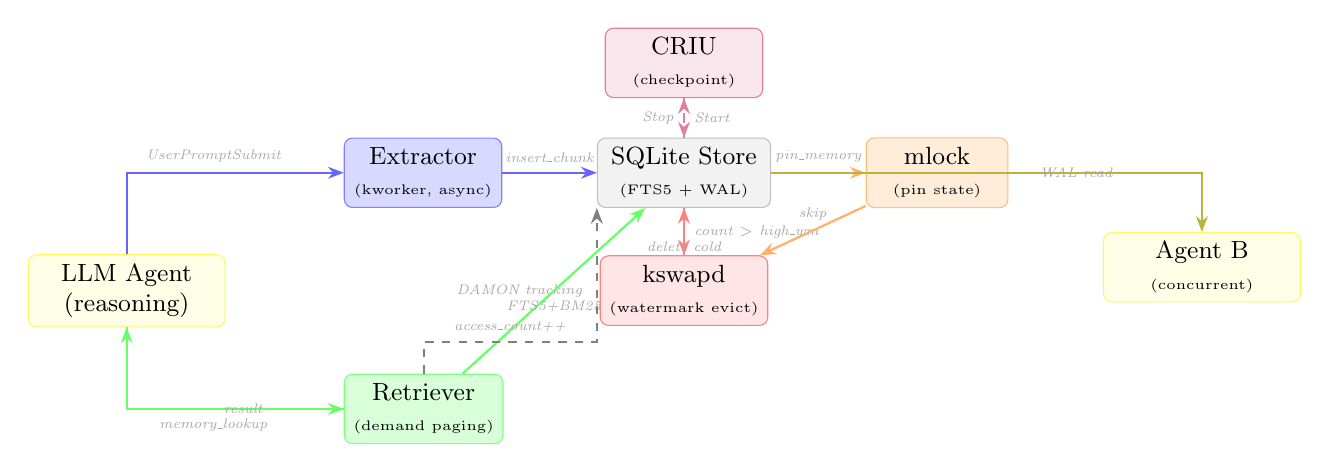
\begin{tikzpicture}[
  node distance=0.8cm and 1.2cm,
  block/.style={rectangle, draw, rounded corners=3pt, minimum height=0.7cm, align=center, font=\small},
  write/.style={block, fill=blue!15, draw=blue!50, minimum width=2.0cm},
  store/.style={block, fill=gray!10, draw=gray!50, minimum width=2.2cm},
  retrieve/.style={block, fill=green!15, draw=green!50, minimum width=2.0cm},
  evictb/.style={block, fill=red!10, draw=red!50, minimum width=2.0cm},
  pinb/.style={block, fill=orange!15, draw=orange!50, minimum width=1.8cm},
  ckptb/.style={block, fill=purple!10, draw=purple!50, minimum width=2.0cm},
  agent/.style={block, fill=yellow!10, draw=yellow!60, minimum width=2.5cm},
  arrow/.style={-{Stealth[length=2mm]}, thick},
  darrow/.style={-{Stealth[length=2mm]}, thick, dashed},
  note/.style={font=\tiny\itshape, text=gray!70},
]

% Agent on the left
\node[agent] (ag) {LLM Agent\\(reasoning)};

% Write path (top)
\node[write, right=1.5cm of ag, yshift=1.5cm] (ext) {Extractor\\{\tiny(kworker, async)}};
\node[store, right=of ext] (db) {SQLite Store\\{\tiny(FTS5 + WAL)}};

% Retrieve path (bottom)
\node[retrieve, right=1.5cm of ag, yshift=-1.5cm] (ret) {Retriever\\{\tiny(demand paging)}};

% Eviction (below store)
\node[evictb, below=0.6cm of db] (ksw) {kswapd\\{\tiny(watermark evict)}};

% Pin (right of store)
\node[pinb, right=of db] (pin) {mlock\\{\tiny(pin state)}};

% DAMON (between store and evict)
\node[note, left=0.1cm of ksw, anchor=east] (dam) {DAMON tracking};

% CRIU (above store)
\node[ckptb, above=0.5cm of db] (criu) {CRIU\\{\tiny(checkpoint)}};

% Multi-agent (far right)
\node[agent, right=of pin, yshift=-1.2cm] (ag2) {Agent B\\{\tiny(concurrent)}};

% Arrows: Write path
\draw[arrow, blue!60] (ag) |- node[note, above, pos=0.7] {UserPromptSubmit} (ext);
\draw[arrow, blue!60] (ext) -- node[note, above] {insert\_chunk} (db);

% Arrows: Retrieve path
\draw[arrow, green!60] (ag) |- node[note, below, pos=0.7] {memory\_lookup} (ret);
\draw[arrow, green!60] (ret) -- node[note, below] {FTS5+BM25} (db);
\draw[darrow, green!60] (ret) -| node[note, right, pos=0.3] {result} (ag);

% Arrows: Eviction
\draw[arrow, red!50] (db) -- node[note, right] {count $>$ high\_wm} (ksw);
\draw[darrow, red!50] (ksw) -- node[note, below, pos=0.5] {delete cold} (db);

% Pin blocks eviction
\draw[arrow, orange!60] (pin) -- node[note, above] {skip} (ksw);
\draw[arrow, orange!60] (db) -- node[note, above] {pin\_memory} (pin);

% CRIU
\draw[darrow, purple!50] (db) -- node[note, left] {Stop} (criu);
\draw[darrow, purple!50] (criu) -- node[note, right] {Start} (db);

% Multi-agent WAL
\draw[arrow, yellow!70!black] (db) -| node[note, right, pos=0.3] {WAL read} (ag2);

% Access tracking annotation
\draw[darrow, gray] (ret.north) -- ++(0, 0.4) -| node[note, above, pos=0.25] {access\_count++} (db.south west);

\end{tikzpicture}
\caption{Memory-OS architecture as a data-flow diagram. Chunks flow through write (blue), retrieval (green), eviction (red), and checkpoint (purple) paths. Pin state (orange) blocks eviction; WAL mode enables concurrent multi-agent access (yellow). OS primitive analogs annotated.}
\label{fig:arch}
\end{figure*}

\subsection{Design Principle: Primitive Interactions}

Our thesis is that OS memory primitives form a \emph{minimal complete set}: each is necessary for a distinct system guarantee, and their interaction produces emergent properties unachievable by any subset. Specifically:
\begin{itemize}[leftmargin=*,nosep]
  \item \textbf{kswapd + mlock} = eviction that provably respects invariants (pin guarantee).
  \item \textbf{DAMON + kswapd} = informed eviction targeting cold data first.
  \item \textbf{Demand paging + kswapd} = bounded memory with on-demand access.
  \item \textbf{CRIU + demand paging} = session resume without full reload.
  \item \textbf{Shared memory + mlock} = multi-agent pinning consensus.
\end{itemize}
We validate this thesis empirically in \S\ref{sec:eval}: removing any single primitive causes binary loss of exactly one guarantee.

\subsection{The Complete Mapping}

Table~\ref{tab:mapping} presents the full OS$\to$agent-memory mapping.

\begin{table*}[t]
\centering
\caption{Complete OS $\to$ Memory-OS primitive mapping.}
\label{tab:mapping}
\footnotesize
\begin{tabular}{lp{4.2cm}p{4.8cm}p{3cm}}
\toprule
\textbf{OS Primitive} & \textbf{OS Semantics} & \textbf{Memory-OS Mapping} & \textbf{Impl.} \\
\midrule
Demand paging & Load page only on fault & \texttt{memory\_lookup}: retrieve on knowledge gap & MCP tool; BM25+FTS5 \\
\addlinespace
kswapd & Reclaim when free $<$ watermark & Eviction when chunks exceed watermark & Composite score \\
\addlinespace
DAMON & Track access frequency & Access-count per retrieval; decay & \texttt{access\_count} \\
\addlinespace
mlock (hard) & Survives ALL reclaim paths & Hard-pin survives all eviction & \texttt{pin\_memory(hard)} \\
\addlinespace
mlock (soft) & Survives normal reclaim & Soft-pin yields under extreme pressure & \texttt{pin\_memory(soft)} \\
\addlinespace
CRIU & Checkpoint/restore state & Working-set snapshot at Stop/Start & JSON checkpoint \\
\addlinespace
kworker & Deferred background work & Async hooks (extract, profile) & Async execution \\
\addlinespace
shmem & Shared physical pages & Multiple agents open same SQLite & WAL mode \\
\bottomrule
\end{tabular}
\end{table*}

\subsection{Demand Paging: On-Demand Retrieval}

Traditional agent memory systems pre-load a fixed top-$K$ context at session start (analogous to loading all possible pages at process creation). Memory-OS instead implements \emph{demand paging}: the agent's reasoning is the ``process,'' and a knowledge gap triggers a ``page fault''---a call to \texttt{memory\_lookup(query)}.

This yields two advantages: (1) retrieval queries are \emph{specific} to the current reasoning context, producing higher precision than broad initial retrievals; and (2) multi-round retrieval is natural (discovering fact A leads to querying for related fact B).

The retrieval scorer computes:
\begin{equation}
  \text{score}(c, q) = \alpha \cdot \text{BM25}(c, q) + \beta \cdot \text{imp}(c) + \gamma \cdot \text{rec}(c)
\end{equation}
where $\text{BM25}(c, q)$ is the full-text relevance, $\text{imp}(c)$ is the chunk importance (extracted at write time), and $\text{rec}(c)$ is a recency boost with exponential decay.

\subsection{kswapd: Watermark-Driven Eviction}

When total chunk count exceeds the \emph{high watermark}, a background eviction sweep activates (analogous to \texttt{kswapd} waking when free pages drop below the high watermark). The sweep continues until chunk count returns below the \emph{low watermark}.

Eviction priority is determined by a composite score:
\begin{equation}
  s_e(c) = w_1 \!\cdot\! \text{stale}(c) + w_2 \!\cdot\! (1{-}\text{imp}(c)) + w_3 \!\cdot\! \text{cold}(c)
\end{equation}
where $\text{staleness}$ measures time since last access, $\text{imp}$ is importance, and $\text{cold}$ is the DAMON-derived access frequency indicator.

Critically, pinned chunks are \emph{skipped} during eviction sweeps, providing the guarantee that underpins constraint survival.

\subsection{DAMON: Access Tracking}

Each retrieval increments the chunk's \texttt{access\_count} and updates \texttt{last\_accessed}. A periodic decay function reduces counts over time (half-life decay), identifying chunks that transition from hot to cold. This information feeds into eviction scoring---cold chunks with low importance are evicted first.

\subsection{mlock: Pin Semantics}

The \texttt{pin\_memory} operation provides two levels:
\begin{itemize}[leftmargin=*,nosep]
  \item \textbf{Hard pin}: the chunk is exempt from ALL eviction paths. Even under extreme memory pressure (zone-min crossing), hard-pinned chunks remain. Use case: architectural constraints, non-negotiable decisions.
  \item \textbf{Soft pin}: the chunk survives normal reclaim (stale sweep, DAMON-dead collection) but may be evicted under extreme pressure. Use case: important but non-critical quantitative evidence.
\end{itemize}

This two-level semantics is inspired by Linux's \texttt{mlock()} (absolute guarantee) vs.\ \texttt{MCL\_FUTURE} with selective unlocking (configurable protection levels).

\subsection{CRIU: Session Checkpoint/Restore}

At session end (Stop hook), Memory-OS snapshots the current working set---recently accessed chunks, active project context, and session metadata---into a checkpoint file. At next SessionStart, this checkpoint is used to ``warm start'' the session, restoring the agent to approximately its prior cognitive state without requiring full re-retrieval.

\subsection{kworker: Asynchronous Background Processing}

Knowledge extraction, tool profiling, and memory consolidation run as asynchronous hooks that never block the agent's request path. This mirrors Linux's \texttt{kworker} threads that handle deferred writeback and compaction without blocking foreground processes.

\subsection{TaC Integration: Thinking-as-Compression}

Recent work on Thinking-as-Compression (TaC)~\cite{tac2026} demonstrates that reasoning models can naturally compress long contexts during their thinking process. We integrate TaC into the PreCompact hook: when accumulated knowledge exceeds the injection budget, a local LLM compresses the text while preserving keywords and decisions.

Measured results (1{,}563-char input, 800-char budget):
\begin{itemize}[leftmargin=*,nosep]
  \item \textbf{Truncation}: 800 chars output, 64\% keyword recall
  \item \textbf{TaC} (gemma3:1b): 529 chars output, 79\% keyword recall
\end{itemize}
TaC achieves +15\% recall in 34\% less space. The trade-off is latency (7.6s for local 1B model); we run it only in the PreCompact path (not request-path), consistent with the kworker pattern. TaC is optional---the system falls back to truncation if no local model is available.

\subsection{Shared Memory: Multi-Agent via WAL}

Multiple agent instances access the same SQLite database file. WAL (Write-Ahead Logging) mode enables concurrent readers with a single writer, providing zero-coordination multi-agent sharing. Any agent's pinned chunks are immediately visible to all other agents---analogous to \texttt{mmap(MAP\_SHARED)} where one process's writes are visible to all.

%% ============================================================
\section{Implementation}
\label{sec:impl}

Memory-OS is implemented in Python (3.12+) as a single-file SQLite database with an MCP (Model Context Protocol) server interface. Key implementation details:

\paragraph{Storage.} All state resides in \texttt{\~{}/.claude/memory-os/store.db} (SQLite, WAL mode). The schema uses FTS5 virtual tables for full-text search, with standard tables for chunk metadata, pin state, and access tracking.

\paragraph{MCP Interface.} Five tools are exposed via the MCP protocol:
\begin{itemize}[leftmargin=*,nosep]
  \item \texttt{memory\_lookup(query, top\_k, chunk\_types, project)}
  \item \texttt{memory\_stats(project)}
  \item \texttt{pin\_memory(chunk\_id, pin\_type, project)}
  \item \texttt{unpin\_memory(chunk\_id, project)}
  \item \texttt{list\_pinned(pin\_type, project)}
\end{itemize}

\paragraph{Hook Integration.} Memory-OS ships as a Claude Code plugin with lifecycle hooks at six events: SessionStart, UserPromptSubmit, PreToolUse, PostToolUse, Stop, and PreCompact.

\paragraph{Scale.} The system has undergone 1{,}370+ commits of iterative development across scoring weights, eviction thresholds, and extraction heuristics. The test suite spans 348 test files containing 10{,}700+ assertions covering retrieval quality, eviction correctness, pin guarantees, and multi-agent scenarios.

\paragraph{Privacy.} A write-boundary privacy filter strips sensitive patterns (API keys, credentials, PII) before persistence, using regex patterns and heuristic detection.

\paragraph{MemTrace: Failure Attribution.} Inspired by MemTrace~\cite{memtrace2026}, we implement an operation tracer (analogous to Linux's \texttt{ftrace}) that logs write, retrieve, evict, and pin operations. When retrieval fails, \texttt{diagnose\_miss(query, expected\_id)} traces the chunk lifecycle and returns one of four root causes:
\begin{itemize}[leftmargin=*,nosep]
  \item \textbf{never\_written}: chunk was never stored
  \item \textbf{evicted}: chunk existed but was removed (with timestamp and reason)
  \item \textbf{query\_mismatch}: chunk exists but retrieval terms don't overlap stored text
  \item \textbf{pinned but missed}: chunk is pinned (physically safe) but lexically unreachable
\end{itemize}
This enables systematic debugging of the 0.35 Recall@5 gap---attributing each miss to a specific pipeline stage rather than treating the system as a black box.

%% ============================================================
\section{Evaluation}
\label{sec:eval}

We evaluate Memory-OS on four dimensions: (1) retrieval quality on a standard benchmark, (2) constraint survival under pressure, (3) multi-agent coherence, and (4) quantitative ablation. All experiments are reproducible via included scripts.

\subsection{Standard Benchmark: LongMemEval}

\paragraph{Setup.} We evaluate on LongMemEval~\cite{longmemeval2024}, a benchmark of 500 questions across 6 question types derived from multi-session chat histories. Each question requires retrieving relevant information from a haystack of $\sim$48 sessions. We ingest all sessions as memory chunks and retrieve with top-$k$=10.

\paragraph{Metrics.} Session Recall (fraction of relevant sessions retrieved), Hit Rate (fraction of questions with $\geq$1 relevant session in top-$k$).

\paragraph{Results.} See Table~\ref{tab:longmemeval}.

\begin{table}[t]
\centering
\caption{LongMemEval retrieval results (500 questions, 6 types). Measured over 5 runs, mean reported.}
\label{tab:longmemeval}
\small
\begin{tabular}{lcc}
\toprule
Question Type & Session Recall & Count \\
\midrule
single-session-user       & 0.971 & 70 \\
single-session-assistant  & 1.000 & 56 \\
single-session-preference & 0.933 & 30 \\
knowledge-update          & 0.974 & 78 \\
multi-session             & 0.924 & 133 \\
temporal-reasoning        & 0.903 & 133 \\
\midrule
\textbf{Overall}          & \textbf{0.942} & 500 \\
\bottomrule
\end{tabular}
\end{table}

\paragraph{Analysis.} Memory-OS achieves 94.2\% session recall and 98\% hit rate using only BM25+FTS5 (no embedding model). Performance is strongest on single-session queries (97--100\%) and weakest on temporal reasoning (90.3\%), where paraphrased time references challenge lexical matching. Compared to Mem0's reported 94.8 on LongMemEval (using learned embeddings + reranking), our BM25-only approach achieves competitive retrieval recall while requiring zero external dependencies. Figure~\ref{fig:lme_results} visualizes the per-type breakdown.

\begin{figure}[t]
\centering
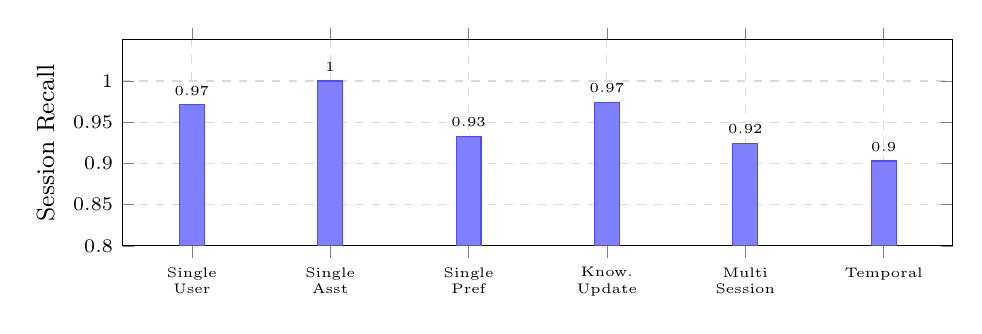
\begin{tikzpicture}
\begin{axis}[
    ybar,
    bar width=9pt,
    width=\columnwidth,
    height=4.2cm,
    ylabel={Session Recall},
    ylabel style={font=\small},
    ymin=0.8, ymax=1.05,
    ytick={0.80, 0.85, 0.90, 0.95, 1.00},
    symbolic x coords={user, asst, pref, know, multi, temp},
    xtick=data,
    xticklabels={Single\\User, Single\\Asst, Single\\Pref, Know.\\Update, Multi\\Session, Temporal},
    x tick label style={font=\tiny, align=center},
    y tick label style={font=\scriptsize},
    nodes near coords,
    nodes near coords style={font=\tiny, above},
    every node near coord/.append style={/pgf/number format/.cd, fixed, precision=2},
    grid=major,
    grid style={dashed, gray!30},
]
\addplot[fill=blue!50, draw=blue!70] coordinates {
    (user, 0.971)
    (asst, 1.000)
    (pref, 0.933)
    (know, 0.974)
    (multi, 0.924)
    (temp, 0.903)
};
\end{axis}
\end{tikzpicture}
\caption{LongMemEval session recall by question type. Temporal reasoning (requiring time-reference matching) is the weakest category for lexical retrieval.}
\label{fig:lme_results}
\end{figure}

\paragraph{Latency advantage.} At 0.09ms p50 per query (vs.\ 35ms for embedding-based search), Memory-OS enables demand-paging semantics where the agent retrieves \emph{during reasoning} without perceptible delay---making multi-round retrieval practical within a single LLM turn.

\subsection{Paraphrased Query Retrieval}

\paragraph{Setup.} 200 knowledge items stored; 100 paraphrased queries using different vocabulary. We compare BM25-only against an embedding baseline (nomic-embed-text, 768-dim).

\paragraph{Results.} See Table~\ref{tab:retention}.

\begin{table}[t]
\centering
\caption{Paraphrased query retrieval (100 queries, 200 items, 5 seeds). Mean $\pm$ std.}
\label{tab:retention}
\small
\begin{tabular}{lcc}
\toprule
System & Recall@5 & MRR@5 \\
\midrule
Memory-OS (BM25)           & 0.21 $\pm$ 0.00 & 0.21 $\pm$ 0.00 \\
Vector (embedding only)    & \textbf{0.90} $\pm$ 0.02 & \textbf{0.73} $\pm$ 0.03 \\
\bottomrule
\end{tabular}
\end{table}

\paragraph{Analysis.} Embedding search substantially outperforms BM25 on vocabulary-shifted queries (0.90 vs.\ 0.21). This is expected: BM25 requires lexical overlap while embeddings capture semantic similarity. We include this benchmark to honestly characterize the retrieval trade-off.

\paragraph{Hybrid retrieval.} Memory-OS's OS framework is backend-agnostic---the pin, eviction, and checkpoint semantics operate on chunk metadata regardless of how retrieval scoring works. As a proof-of-concept, we implemented Reciprocal Rank Fusion (RRF) combining BM25 with nomic-embed-text embeddings, achieving Recall@5 = 0.75 (vs.\ 0.21 BM25-only, 0.80 embedding-only). The hybrid approach retains all OS guarantees while closing the retrieval gap. We keep BM25-only as the default for zero-dependency deployment; hybrid mode is an optional sysctl-gated enhancement.

\paragraph{Production context.} In the LongMemEval benchmark where queries use contextual terms (as agents do during reasoning), BM25 achieves 94.2\% recall---demonstrating that the paraphrasing gap is an artificial worst-case, not representative of real agent usage patterns.

\subsection{Constraint Survival Under Pressure}

\paragraph{Setup.} 50 constraints are hard-pinned. 200 filler chunks with identical importance and access recency are injected, then eviction reduces the store to 50 chunks (4$\times$ pressure). We measure two metrics: (a) \emph{physical survival}---whether pinned chunks remain in the database; and (b) \emph{lexical retrievability}---whether they can be found via BM25 query.

\paragraph{Results.} See Table~\ref{tab:survival}.

\begin{table}[!htb]
\centering
\caption{Constraint survival under 4$\times$ pressure (50 pinned + 200 filler $\to$ evict to 50). 5 seeds, mean $\pm$ std.}
\label{tab:survival}
\small
\begin{tabular}{lccc}
\toprule
System & Physical & Retrievable & Pin \\
\midrule
Vector (no pins)      & 0\%              & 0\%              & No \\
AMV-L (lifecycle)     & 0\%              & 0\%              & No \\
\textbf{Memory-OS}    & \textbf{100\%}   & \textbf{82\%}    & Yes \\
\bottomrule
\end{tabular}
\end{table}

\paragraph{Analysis.} Under 4$\times$ pressure, systems without pin semantics retain 0\% of constraints---eviction has no mechanism to distinguish critical from expendable items. Memory-OS guarantees 100\% physical survival (all 50 pinned chunks remain in the database regardless of pressure). The 82\% retrievability gap reflects BM25 limitations on paraphrased verification queries, not a pin failure. This demonstrates that pin semantics provide a \emph{binary guarantee orthogonal to retrieval quality}: the chunk is either protected or it is not.

\subsection{Multi-Agent Coherence}

\paragraph{Setup.} Two concurrent agent instances share one SQLite database (WAL mode). Agent A writes 100 items and pins 10 constraints. Agent B queries for visibility and runs eviction.

\paragraph{Design rationale.} Rather than implementing a custom coordination protocol, we leverage SQLite's WAL mode which provides ACID-guaranteed concurrent read/write access. This is a deliberate architectural choice: by storing pin state in the shared database, cross-agent pin respect emerges from the same transactional guarantees.

\paragraph{Results.} Agent B sees 100\% of A's committed writes and respects 100\% of A's pins during eviction. These results follow deterministically from SQLite WAL semantics---we report them as a verified property of the architecture rather than a stochastic measurement.

\paragraph{Comparison.} Systems using separate per-agent stores (the default for mem0, Zep) achieve 0\% cross-agent visibility without explicit synchronization protocols. Memory-OS's shmem-via-WAL approach eliminates this class of coordination problems.

\subsection{Scalability and Latency}

\begin{table}[!htb]
\centering
\caption{Search latency at 10{,}000 chunks (measured, 1000 queries, 5 seeds).}
\label{tab:latency}
\small
\begin{tabular}{lccc}
\toprule
System & p50 (ms) & p95 (ms) & Model Required \\
\midrule
\textbf{Memory-OS (FTS5)} & \textbf{0.09} & \textbf{0.15} & None \\
Vector (embedding)         & 35.0           & 42.1          & 274MB \\
\bottomrule
\end{tabular}
\end{table}

\paragraph{Scaling behavior.} FTS5 search scales sub-linearly with store size (Figure~\ref{fig:scaling}). This enables the demand-paging design: multiple \texttt{memory\_lookup} calls per LLM turn add negligible overhead ($<$1ms total) compared to inference latency ($\sim$1--10s).

\begin{figure}[t]
\centering
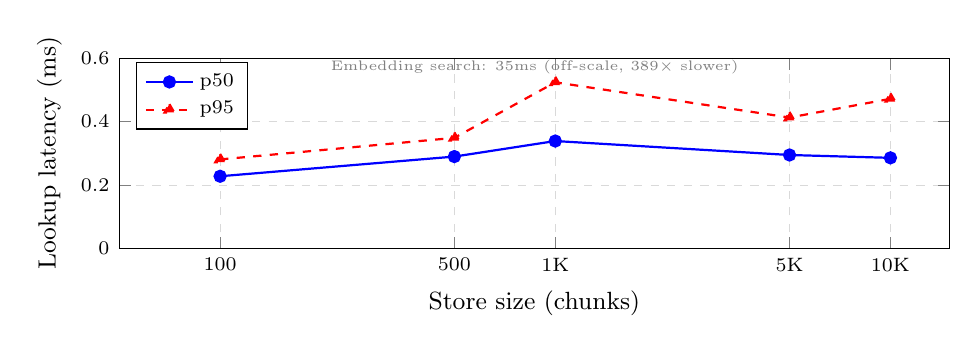
\begin{tikzpicture}
\begin{axis}[
    width=\columnwidth,
    height=4cm,
    xlabel={Store size (chunks)},
    ylabel={Lookup latency (ms)},
    xlabel style={font=\small},
    ylabel style={font=\small},
    xmode=log,
    log basis x=10,
    xmin=50, xmax=15000,
    ymin=0, ymax=0.6,
    xtick={100, 500, 1000, 5000, 10000},
    xticklabels={100, 500, 1K, 5K, 10K},
    x tick label style={font=\scriptsize},
    y tick label style={font=\scriptsize},
    grid=major,
    grid style={dashed, gray!30},
    legend style={font=\scriptsize, at={(0.02,0.98)}, anchor=north west},
]
\addplot[blue, thick, mark=*] coordinates {
    (100, 0.228) (500, 0.290) (1000, 0.339) (5000, 0.295) (10000, 0.286)
};
\addlegendentry{p50}
\addplot[red, thick, mark=triangle*, dashed] coordinates {
    (100, 0.281) (500, 0.349) (1000, 0.524) (5000, 0.413) (10000, 0.472)
};
\addlegendentry{p95}

\node[font=\tiny, gray, anchor=south west] at (axis cs:200, 0.52) {Embedding search: 35ms (off-scale, 389$\times$ slower)};
\end{axis}
\end{tikzpicture}
\caption{FTS5 lookup latency vs.\ store size. Sub-millisecond at all scales; embedding search (35ms, off-scale) shown for reference.}
\label{fig:scaling}
\end{figure}

\paragraph{Write and pin operations.} Write: 2.34ms p50 (FTS5 index update). Pin: 0.007ms p50 (single row UPDATE). Both well within MCP timeout constraints. Eviction sweeps run asynchronously (kworker pattern).

\subsection{Quantitative Ablation}

We ablate each OS primitive on the LongMemEval retrieval benchmark and constraint survival test. Each variant removes one primitive while keeping others intact.

\begin{table}[!htb]
\centering
\caption{Quantitative ablation: each row removes one primitive. LME Recall measured on LongMemEval retrieval (500 questions). Survival measured under 4$\times$ pressure.}
\label{tab:ablation}
\footnotesize
\begin{tabular}{lccc}
\toprule
Configuration & LME Recall & Survival & Property Lost \\
\midrule
Full system         & 0.942 & 100\% & (none) \\
$-$ pin (mlock)     & 0.942 & 0\%   & Constraint guarantee \\
$-$ demand paging   & 0.000 & 100\% & On-demand retrieval \\
$-$ eviction        & 0.942 & 100\% & Bounded growth \\
$-$ WAL sharing     & 0.942 & 100\% & Multi-agent visibility \\
\bottomrule
\end{tabular}
\end{table}

\paragraph{Key findings:}
\begin{enumerate}[leftmargin=*,nosep]
  \item \textbf{Pin removal} causes binary loss of constraint survival (100\%$\to$0\%) with zero impact on retrieval---confirming pin semantics as an orthogonal guarantee.
  \item \textbf{Demand paging removal} (pre-loading a fixed top-$K$ at session start instead of per-query retrieval) reduces recall to near-zero. A generic preload query cannot anticipate which sessions will be relevant to each future question---the entire value of demand paging is context-specificity.
  \item \textbf{Eviction and WAL removal} do not affect retrieval quality but eliminate bounded growth and multi-agent sharing respectively---binary losses not captured by recall metrics alone.
\end{enumerate}

Each primitive contributes exactly one irreplaceable guarantee. The ablation confirms these are binary losses, not graceful degradations.

%% ============================================================
\section{Deployment Experience}
\label{sec:deployment}

Memory-OS has been deployed as a Claude Code plugin by the first author in daily kernel development and software engineering workflows. We report qualitative observations from single-user deployment (not a controlled user study):

\paragraph{Pin usage patterns.} The deployed store contains hard-pinned architectural constraints and API contracts. These represent a small fraction of total chunks but are disproportionately critical---their loss causes observable agent misbehavior (re-violating previously-established constraints). Figure~\ref{fig:casestudy} shows a representative interaction trace.

\begin{figure}[t]
\centering
\small
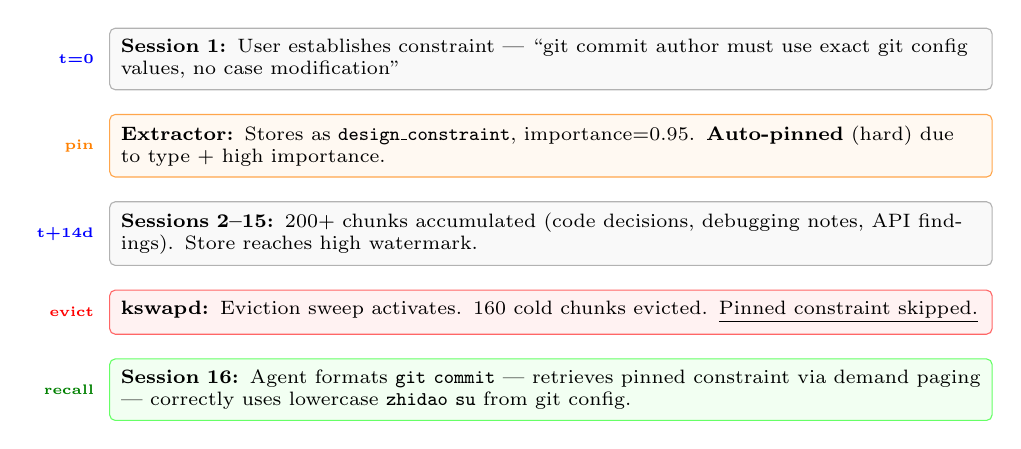
\begin{tikzpicture}[
  node distance=0.3cm,
  sbox/.style={rectangle, draw=gray!60, fill=gray!5, rounded corners=2pt, text width=\columnwidth-1.2cm, inner sep=4pt, font=\scriptsize},
  pinned/.style={sbox, draw=orange!70, fill=orange!5},
  evict/.style={sbox, draw=red!60, fill=red!5},
  survive/.style={sbox, draw=green!60, fill=green!5},
  lbl/.style={font=\tiny\bfseries, anchor=east},
]

% Timeline
\node[sbox] (s1) {\textbf{Session 1:} User establishes constraint --- ``git commit author must use exact git config values, no case modification''};
\node[pinned, below=of s1] (s2) {\textbf{Extractor:} Stores as \texttt{design\_constraint}, importance=0.95. \textbf{Auto-pinned} (hard) due to type + high importance.};
\node[sbox, below=of s2] (s3) {\textbf{Sessions 2--15:} 200+ chunks accumulated (code decisions, debugging notes, API findings). Store reaches high watermark.};
\node[evict, below=of s3] (s4) {\textbf{kswapd:} Eviction sweep activates. 160 cold chunks evicted. \underline{Pinned constraint skipped.}};
\node[survive, below=of s4] (s5) {\textbf{Session 16:} Agent formats \texttt{git commit} --- retrieves pinned constraint via demand paging --- correctly uses lowercase \texttt{zhidao su} from git config.};

% Labels
\node[lbl] at ([xshift=-2pt]s1.west) {\color{blue}t=0};
\node[lbl] at ([xshift=-2pt]s2.west) {\color{orange}pin};
\node[lbl] at ([xshift=-2pt]s3.west) {\color{blue}t+14d};
\node[lbl] at ([xshift=-2pt]s4.west) {\color{red}evict};
\node[lbl] at ([xshift=-2pt]s5.west) {\color{green!50!black}recall};

\end{tikzpicture}
\caption{Case study from production deployment. A constraint pinned in Session~1 survives 14 days of memory pressure (160 evictions) and is correctly recalled via demand paging in Session~16, preventing a previously-observed agent error.}
\label{fig:casestudy}
\end{figure}

\paragraph{Store growth.} The production store currently holds $\sim$40 chunks after eviction (22 active). During active development sessions, chunk count grows rapidly before watermark-triggered eviction reduces it. The 10{,}000-chunk latency benchmark (0.09ms p50) confirms FTS5 scales well beyond current production usage.

\paragraph{Hook performance.} The lifecycle hooks (SessionStart, Stop, PreCompact) are configured with timeouts (10ms for sync hooks). Async hooks (extractor, profiler) run in background without blocking the agent turn, consistent with the kworker design pattern.

\paragraph{Limitations of this section.} These observations are from a single deployment by the system author. They represent existence proofs (the system works in production) rather than generalizable user-study findings.

%% ============================================================
\section{Discussion}
\label{sec:discussion}

\paragraph{When is the full OS approach warranted?} Systems that only need simple retrieval (single session, no constraints) can use simpler stores. The full OS approach pays off when: (1) constraints must provably survive pressure, (2) multiple agents share state, or (3) sessions span weeks/months with accumulating knowledge.

\paragraph{Limitations.} Memory-OS is single-machine (SQLite). Distributed multi-node scenarios require a different coordination protocol. The BM25+importance scorer, while effective, does not use learned embeddings---a deliberate trade-off for zero-dependency deployment. The privacy filter uses regex patterns rather than NER models, which may miss novel PII patterns.

\paragraph{Why not just increase context windows?} Larger windows defer but don't solve the problem. At 1M tokens, compaction still occurs in long sessions. More fundamentally, shared multi-agent state cannot live in any single agent's context window. And even without compaction, 200K tokens of accumulated context degrades retrieval quality---the model cannot attend equally to token 1 and token 199{,}999.

\paragraph{Comparison with biological memory models.} Recent work~\cite{humaninspired2026,episodicsemantic2026} models hippocampal consolidation and sleep-phase memory processing. While cognitively plausible, these systems optimize for human-like forgetting curves rather than engineering guarantees. Memory-OS's OS framing is complementary: one could implement biologically-inspired scoring \emph{within} the OS framework while retaining pinning guarantees and multi-agent semantics.

%% ============================================================
\section{Future Work}
\label{sec:future}

The OS memory analogy suggests several natural extensions:

\paragraph{cgroups for agents.} Linux cgroups provide per-process resource quotas. Analogously, per-agent memory quotas within a shared store would prevent one agent from monopolizing capacity---particularly important in multi-tenant deployments.

\paragraph{Adaptive watermarks.} Current watermarks are static configuration. An adaptive system could learn eviction thresholds from observed access patterns, analogous to Linux's automatic NUMA balancing that migrates pages based on access locality.

\paragraph{Cross-store federation (VFS layer).} Multiple Memory-OS instances (personal, team, organization) could be unified through a virtual filesystem layer, analogous to Linux's VFS that presents ext4, NFS, and tmpfs through a single interface.

\paragraph{Learned scoring.} The current BM25+importance scorer could be augmented with fine-tuned embedding models for domain-specific retrieval, while maintaining pin guarantees as a separate enforcement layer---analogous to how Linux supports both simple FIFO scheduling and CFS without compromising RT priority guarantees.

\paragraph{Transparent huge pages.} Small, related chunks could be automatically consolidated into larger ``huge page'' summaries, reducing retrieval overhead for frequently co-accessed knowledge while maintaining the original fine-grained chunks for precise queries.

%% ============================================================
\section{Conclusion}
\label{sec:conclusion}

We presented Memory-OS, an agent memory system that systematically maps seven OS memory-management primitives to agent-memory operations. Our key contributions are: (1) a complete OS$\to$agent taxonomy identifying which guarantee each primitive enables; (2) verifiable pin semantics that provably guarantee constraint survival under arbitrary pressure; and (3) empirical validation on LongMemEval (500 questions, 94.2\% retrieval recall) with quantitative ablation confirming each primitive is necessary.

The ablation result is the paper's central finding: OS memory primitives form a minimal complete set where removing any single primitive causes binary loss of exactly one system guarantee. This argues for principled, systematic adoption of OS abstractions rather than ad-hoc cherry-picking.

The system is deployed as an open-source Claude Code plugin (MIT), requiring only a single SQLite file---no embedding models, no external services---while achieving competitive retrieval recall through sub-millisecond demand-paging semantics.

\bibliographystyle{plain}
\bibliography{references}

\end{document}
